\section{Background}
\label{section:bbc:background}

\begin{lstlisting}[frame=tb,
    caption={Method \texttt{fromMap} from XWIKI version 8.1 (collected in Chapter \ref{sec:jcrashpack:introduction})},
    label=list:fromMap,
    language=java,
    captionpos=t,
    numbers=left,
    basicstyle=\tiny,
    belowskip=-2.5em,
    float=t,
    firstnumber=402]
    public BaseCollection fromMap(Map<[...]> map, BaseCollection object){
        for (PropertyClass property : (Collection<[...]>) getFieldList()) {
            String name = property.getName();
            Object formvalues = map.get(name);
            if (formvalues != null) {
                BaseProperty objprop;
                if (formvalues instanceof String[]) {
                    [...]
                } else if (formvalues instanceof String) {
                    objprop = property.fromString(formvalues.toString());
                } else {
                    objprop = property.fromValue(formvalues);
                }
                [...]
            }}
        return object;}
  \end{lstlisting}
 
  \begin{figure}[t]
    \centering
    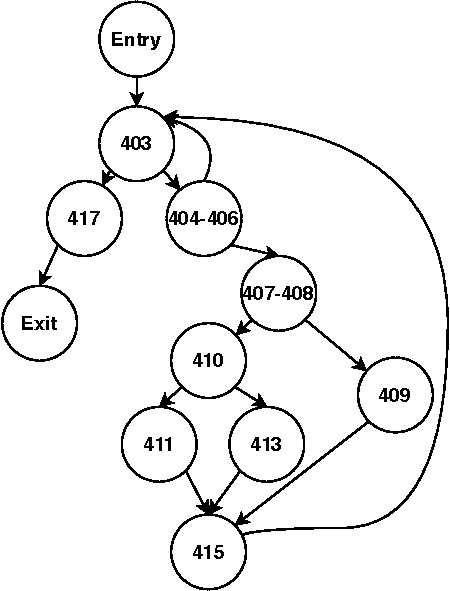
\includegraphics[width=0.35\linewidth]{papers/bbc/figures/fromMapCFG}
    
    \caption{CFG for method \texttt{fromMap}}
  \label{fig:CFG}
\end{figure}

\subsection{Coverage Distance Heuristics}
\label{section:background:distance}

Many structural-based search-based test generation approaches mix the \textit{branch distance} and \textit{approach level} heuristics to achieve a high line and branch coverage~\cite{McMinn2004}. These heuristics measure the distance between a test execution path and a specific statement or a specific branch in the software under test.
For that, they rely on the coverage information of \emph{control dependent basic blocks}, \ie basic blocks that have at least one outgoing edge leading the execution path toward the \emph{target basic block} (containing the targeted statement) and at least another outgoing edge leading the execution path away from the target basic block.
As an example, Listing \ref{list:fromMap} shows the source code of method \texttt{fromMap} in XWIKI\footnote{https://github.com/xwiki}, and Figure \ref{fig:CFG} contains the corresponding CFG. In this graph, the basic block \texttt{409} is control dependent on the basic block \texttt{407-408} because the execution of line 409 is dependent on the satisfacation of the predicate at line 408 (\ie line 409 will be executed only if elements of array \texttt{formvalues} are \texttt{String}).

The \textit{approach level} is the number of uncovered control dependent basic blocks for the target basic block between the closest covered control dependent basic block and the target basic block. The \textit{branch distance} is calculated from the predicate of the closest covered control dependent basic block, based on a set of predefined rules. Assuming that the test $t$ covers only line \texttt{403} and \texttt{417}, and our target line is \texttt{409}, the approach level is 2 because two control dependent basic blocks (\texttt{404-406} and \texttt{407-408}) are not covered by $t$. The branch distance the predicate in line \texttt{403} (the closest covered control dependency of node \texttt{409}) is measured based on the rules from the establised technique \cite{McMinn2004}.

To the best of our knowledge, there is no related work studying the extra heuristics helping the combination of approach level and branch distance to improve the coverage. Most related to our work, Panichella \etal \cite{Panichella2018} and Rojas \etal \cite{rojas2015combining} introduced two heuristics called \textit{infection distance} and \textit{propagation distance}, to improve the weak mutation score of two generated test cases. However, these heuristics do not help the search process to improve the general statement coverage (\ie they are effective only after covering a mutated statement).

In this paper, we introduce a new secondary objective to improve the statement coverage achieved by fitness functions based on the approach level and branch distance, and analyze the impact of this secondary objective on \textbf{search-based crash reproduction}.

% \begin{figure}[t]
    \begin{lstlisting}[
        caption=XWIKI-13377 crash stack trace (collected in Chapter \ref{sec:jcrashpack:introduction}),
        label=lst:stacktrace,
        numbers=left,
        firstnumber=0,
        belowskip=-1.5em
        ]
java.lang.ClassCastException: [...]
    at [...].BaseStringProperty.setValue(BaseStringProperty.java:45)
    at [...].PropertyClass.fromValue(PropertyClass.java:615)
    at [...].BaseClass.fromMap(BaseClass.java:413)
    [...] (*@\label{line:bbc:lowestframe}@*)
    \end{lstlisting}
% \end{figure}

\subsection{Search-based Crash Reproduction}

After a crash is reported, one of the essential steps of software debugging is to write a \textbf{Crash Reproducing Test case (\CRT)} to make the crash observable to the developer and help them in identifying the root cause of the failure \cite{Zeller2009}. Later, this \CRT can be integrated into the existing test suite to prevent future regressions. Despite the usefulness of a \CRT, the process of writing this test can be labor-intensive and time-taking \cite{Soltani2018a}. 
Various techniques have been introduced to automate the reproduction of a crash \cite{Chen2015, Xuan2015, nayrolles2015jcharming, Rossler2013, Soltani2018a}, and search-based approaches (\evocrash \cite{Soltani2018a} and \recore \cite{Rossler2013}) yielded the best results~\cite{Soltani2018a}.


\textbf{\evocrash.}
This approach utilizes a single-objective genetic algorithm to generate a \CRT from a given stack trace and a \textit{target frame} (\ie a frame in the stack trace that its class will be used as the class under test). The \CRT generated by \evocrash throws the same stack trace as the given one up to the target frame. 
For example, by passing the stack trace in Listing~\ref{lst:stacktrace} and target frame 3 to \evocrash, it generates a test case reproducing the first three frames of this stack trace (\ie thrown stack trace is identical from line 0 to 3).

\evocrash uses a fitness function, called \WS, to evaluate the candidate test cases. \WS is the sum scalarization of three components:
\begin{inparaenum}[(i)]
    \item the \textbf{target line coverage} ($d_{s}$), which measures the distance between the execution trace and the \textit{target line} (\ie the line number pointed to by the target frame) using \textit{approach level} and \textit{branch distance};
    \item the \textbf{exception type coverage}  ($d_{e}$), determining whether the type of the triggered exception is the same as the given one; and 
   \item the \textbf{stack trace similarity}  ($d_{tr}$), which indicates whether the stack trace triggered by the generated test contains all frames (from the most in-depth frame up to the target frame) in the given stack trace.
   \end{inparaenum}

   \begin{definition}[\WS \cite{Soltani2018a}]
    For a given test case execution $t$, the \WS ($ws$) is defined as follows:
    \begin{equation}
    \small
    ws(t) = 
    \left\{
        \begin{array}{ll}
          3 \times d_{s}(t) + 2 \times max(d_{e}) + max(d_{tr}) & \textit{ if line not reached}\\
          3 \times min(d_{s}) + 2 \times d_{e}(t) + max(d_{tr}) & \textit{if line reached}\\
          3 \times min(d_{s}) + 2 \times min(d_{e}) + d_{tr}(t) & \textit{if exception thrown}
        \end{array}
      \right.
     \end{equation}
    \end{definition}
%
Where $d_{s}(t) \in [0,1]$ indicates how far $t$ is from reaching the target line and is computed using the normalized approach level and branch distance: $d_{s}(t) = \Vert approachLevel_{s}(t)  + \Vert branchDistance_{s}(t)\Vert\Vert$. 
Also, $d_{e}(t) \in \{0,1\}$ shows if the type of the exception thrown by $t$ is the same as the given stack trace ($0$) or not ($1$). Finally, $d_{tr}(t) \in [0,1]$ measures the stack trace similarity between the given stack trace and the one thrown by $t$. $max(f)$ and $min(f)$ denote the maximum and minimum possible values for a function $f$, respectively.
In this fitness function, $d_{e}(t)$ and $d_{tr}(t)$ are only considered in the satisfaction of two \textit{constraints}: (i) \textit{exception type coverage} is relevant only 
when we reach the target line and (ii) \textit{stack trace similarity} is important only when we both reach the target line and throw the same type of exception.

As an example, when applying \evocrash on the stack trace from Listing~\ref{lst:stacktrace} with the target frame 3, \WS first checks if the test cases generated by the search process reach the statement pointed to by the target frame (line 413 in class \texttt{BaseClass} in this case). Then, it checks if the generated test can throw a \texttt{ClassCastException} or not. Finally, after fulfilling the first two constraints, it checks the similarity of frames in the stack trace thrown by the generated test case against the given stack trace in Listing~\ref{lst:stacktrace}. 

% \evocrash uses a guided genetic algorithm to ensure that any test case generated during the search process contains, at least, one method call to the \textit{target method} (\ie method appeared in the target frame). In the \textbf{search initialization}, \evocrash generates random test cases that have at least one method call to the target method. Next, in each generation, \evocrash evolves the fittest test cases using \textbf{guided mutation} (a classical mutation while ensuring that the evolved test case has one or more target method calls) and \textbf{guided crossover} (a single-point crossover that keeps the target method calls in the offsprings).

\evocrash uses \textbf{guided} initialization, mutation and single-point crossover operators to ensure that the target method  (\ie the method appeared in the target frame) is always called by the different tests during the evolution process. 

% A recent study \cite{Soltani2018a} draws a comparison between all of the approaches that use only stack traces to reproduce a crash. According to its results, \evocrash outperforms other non-search-based crash reproduction approaches in terms of \textit{effectiveness in crash reproduction} and \textit{efficiency}. This study also shows the helpfulness of tests generated by \evocrash for developers during debugging. 

According to a recent study, \evocrash outperforms other non-search-based crash reproduction approaches in terms of \textit{effectiveness in crash reproduction} and \textit{efficiency}~\cite{Soltani2018a}. This study also shows the helpfulness of tests generated by \evocrash for developers during debugging. 

In this paper, we assess the impact of \bbc as the secondary objective in the \evocrash search process.


\textbf{\recore.}
This approach utilizes a genetic algorithm guided by a single fitness function, which has been defined according to the core dump and the stack trace produced by the system when the crash happened. To be more precise,  this fitness function is a sum scalarization of three sub-functions: (i) \textbf{TestStackTraceDistance}, which guides the search process according to the given stack trace; (ii) \textbf{ExceptionPenalty}, which indicates whether the same type of exception as the given one is thrown or not (identical to ExceptionCoverage in \evocrash); and (iii) \textbf{StackDumpDistance}, which guides the search process by the given core dump. 
\begin{definition}[\textit{TestStackTraceDistance} \cite{Rossler2013}]
    For a given test case execution $t$, the \textit{TestStackTraceDistance} ($STD$) is defined as follows:
    \begin{equation}
    \small
    STD(R,t) = |R| - lcp - (1-StatementDistance(s))
     \end{equation}
\end{definition}
%
Where $|R|$ is the number of frames in the given stack trace. And $lcp$ is the longest common prefix frames between the given stack trace and the stack trace thrown by $t$. Concretely, $|R| - lcp$ is the number of frames not covered by $t$. Moreover, $StatementDistance(s)$ is calculated using the sum of the approach level and the normalized branch distance to reach the statement $s$, which is pointed to by the first (the utmost) uncovered frame by $t$: $StatementDistance(s) = approachLevel_{s}(t) + \Vert branchDistance_{s}(t) \Vert$.

Since using runtime data (such as core dumps) can cause significant overhead \cite{Chen2015} and leads to privacy issues \cite{nayrolles2015jcharming}, the performance of \recore in crash reproduction was not compared with \evocrash in prior studies \cite{Soltani2018a}.
Although, two out of three fitness functions in \recore use only the given stack trace to guide the search process. Hence, this study only considers \textit{TestStackTraceDistance} $+$ \textit{ExceptionPenalty} (called \integ hereafter).

As an example, when applying \recore with \integ on the stack trace in Listing~\ref{lst:stacktrace} with target frame 3, first, \integ determines if the generated test covers the statement at frame 3 (line 413 in class \texttt{BaseClass}). Then, it checks the coverage of frame 2 (line 615 in class \texttt{PropertyClass}). After covering the first two frames by the generated test case, it checks the coverage of the statement pointed to by the deepest frame (line 45 in class \texttt{BaseStringProperty}). For measuring the coverage of each of these statements, \integ uses the approach level and branch distance. After covering all of the frames, this fitness function checks if the the generated test throws \texttt{ClassCastException} in the deepest frame.

In this study, we perform an empirical evaluation to assess the performance of crash reproduction using \integ with and without \bbc as the secondary objective in terms of \textit{effectiveness in crash reproduction} and \textit{efficiency}.

% compare the performance of the crash reproduction guided by \integ against \evocrash in terms of \textit{effectiveness in crash reproduction} and \textit{efficiency}. We also analyze the cases that one of these algorithms can achieve a better result compared to the other one. Moreover, we evaluate 

% The former utilizes a genetic algorithm guided by a single fitness function, which has been defined according to the core dump and the stack trace produced by the system when the crash happened. To be more precise,  this fitness function is a sum scalarization of two sub-functions: \integ, which guides the search process according to the given stack trace, and \textit{TestStackDumpDistance}, which guides the search process by the given core dump.
% The latter also uses a guided genetic algorithm with a single objective (called \WS hereafter), which is defined only by the given stack trace.

% Since using runtime data (such as core dumps) can cause significant overhead \cite{Chen2015} and leads to privacy issues \cite{nayrolles2015jcharming}, a recent study \cite{Soltani2018a} compares all of the crash reproduction approaches using only stack traces to fulfill this task. According to the results of this study, \evocrash outperforms other non-search-based crash reproduction approaches in terms of \textit{effectiveness in crash reproduction} (\ie percentage of times that an approach can reproduce a crash) and \textit{efficiency} (\ie time required by an approach for reproducing a crash). This study also shows the helpfulness of \CRT, generated by \evocrash, for developers during debugging. However, there is no comparison between \WS (used by \evocrash for reproducing the crash according to the stack trace) and \integ (used by \recore to reproduce the crash only by the thrown stack trace).

% However, there is no comparison between \WS (used by \evocrash for reproducing the crash according to the stack trace) and \integ (used by \recore to reproduce the crash only by the thrown stack trace).
% In this study, we perform an empirical evaluation to compare \WS against \integ in terms of \textit{effectiveness in crash reproduction} and \textit{efficiency}. We also analyze the cases that one of these algorithms can achieve a better result compared to the other one.


